
\documentclass[a4paper,12pt]{article}
\usepackage[english,russian]{babel}
\usepackage[many]{tcolorbox}
\usepackage[utf8]{inputenc}
\usepackage[T2A]{fontenc}
\usepackage{amssymb}
\usepackage[unicode, pdftex]{hyperref}


\usepackage[
  a4paper, mag=1000, includefoot,
  left=1.1cm, right=1.1cm, top=1.2cm, bottom=1.2cm, headsep=0.8cm, footskip=0.8cm
]{geometry}

\usepackage{amsmath}
\usepackage{amssymb}
\usepackage{times}
\usepackage{mathptmx}
\usepackage{graphicx}
\usepackage{tikz}
\newtheorem{deff}{\textit{Определение}}
\newtheorem{teo}{\textit{Теорема}}
\newtheorem{utv}{\textit{Утверждение}}
\newtheorem{lem}{\textit{Лемма}}
\newtheorem{deff2}{\textit{Определение}}
\newtheorem{teo2}{\textit{Теорема}}
\newtheorem{utv2}{\textit{Утверждение}}
\newtheorem{lem2}{\textit{Лемма}}
\newcommand{\ee}{\equiv}

\newcommand{\pp}{\partial}
\newcommand{\FI}{\varphi}
\newcommand{\TE}{\theta}
\newcommand{\AL}{\alpha}
\newcommand{\SI}{\psi}
\newcommand{\q}{\quad}
\newcommand{\pb}{\blacktriangleright}
\newcommand{\pe}{\blacktriangleleft}
\newcommand{\Ra}{\Rightarrow}
\newcommand{\bb}[1]{\mathbb{#1}}
\newcommand{\dt}{\frac{d}{dt}}
\newcommand{\fracp}[2]{\frac{\pp #1}{\pp #2}}

\newcommand{\pf}{\textit{Доказательство}\\}
\newcommand{\pfe}{\textit{Доказательство окончено}\\}

\newcommand{\SL}{\sum\limits}
\newcommand{\IL}{\int\limits}
\newcommand{\os}{\left(}
\newcommand{\cs}{\right)}
\newcommand{\R}{\mathbb{R}}
\newtcolorbox{mybox}[2][]{
    colback=white,
    colframe=blue!50!black,
    title=#2,
    fonttitle=\bfseries,
    enhanced,
    breakable,
    attach boxed title to top left={yshift=-\tcboxedtitleheight/2},
    boxed title style={size=small,colback=red,colframe=blue!50!black},
    #1
}

\usepackage{blindtext}
\usepackage{titlesec}
\title{ТЧ-8 2024}
\author{SFS}
\date{\today}
\begin{document}
\maketitle


\tableofcontents
\newpage
\section{Билеты}
\begin{enumerate}
\item{Билет 1}
 \hyperlink{bil1}{Простейшие свойства делимости. Представление наибольшего общего делителя $d$ чисел $a$ и $b$ в форме $d = au+bv$. Теорема о существовании и единственности разложения на простые сомножители. Бесконечность множества простых чисел.}
\item{Билет 2}
 \hyperlink{bil2}{Лемма о равенстве верхних и нижних пределов функций ($\TE(x)/x, \SI(x)/x$ и $\os\pi(x)\ln(x)\cs/x$). Связь между асимптотическим поведением функции Чебышева $\SI(x)$ и сходимостью интеграла $$\IL_1^\infty \frac{\SI(x)-x}{x^2}dx$$}

\item{Билет 3}
\hyperlink{bil3}{Оценки Чебышева функции $\pi(x)$. Оценки $n$-го простого числа. Расходимость ряда $\sum_p \frac{1}{p}$.}

\item{Билет 4}
\hyperlink{bil4}{Аналитичность дзета-функции Римана в области $\sigma > 1$. Разложение в ряд Дирихле ее логарифмической производной. Представление дзета-функции в виде бесконечного произведения.}

\item{Билет 5}
\hyperlink{bil5}{Преобразование Абеля в интегральной форме. Аналитическое продолжение дзета-функции в область $\sigma > 0$.}

\item{Билет 6}
\hyperlink{bil6}{Отсутствие нулей дзета-функции в области $\sigma \ge 1$.}

\item{Билет 7}
\hyperlink{bil7}{Формулировка асимптотического закона распределения простых чисел. Сведение его доказательства к исследованию некоторого комплексного интеграла.}

\item{Билет 8}
\hyperlink{bil8}{Доказательство асимптотического распределения распределения простых чисел. Асимптотическая формула $n$-го простого числа.}


\item{Билет 9}
\hyperlink{bil9}{Простейшие свойства сравнений. Группа $\os Z/mZ \cs ^*$. Теорема Эйлера. Малая теорема Ферма. Элементарные доказательства бесконечности множества простых чисел в прогрессиях вида $4n+1$ и $4n+3$.}

\item{Билет 10}
\hyperlink{bil10}{Простейшие свойства групповых характеров. Построение характеров. Вычисление сумм $\sum_{a\in G} \chi(a)$ и $\sum_\chi \chi(a)$ для характеров $\chi$ группы $G$. Определение и свойства числовых характеров.}

\item{Билет 11}
\hyperlink{bil11}{Аналитичность функции Дирихле $L(s,\chi)$ в области $\sigma > 1$. Разложение в ряд Дирихле ее логарифмической производной. Отсутствие нулей $L$-функции в области $\sigma > 1$. Представление $L$-функции в виде бесконечного произведения. Аналитическое продолжение функции $L(s,\chi_0)$ в область $\sigma > 0$.}


\item{Билет 12}
\hyperlink{bil12}{Теорема о почленном дифференцировании ряда Дирихле. Область аналитичности функции $L(s, \chi)$ при $\chi \not= \chi_0$.}

\item{Билет 13}
\hyperlink{bil13}{Теорема об области сходимости ряда Дирихле с неотрицательными коэффициентами.}

\item{Билет 14}
\hyperlink{bil14}{Неравенство $L(1,\chi)\not=0$ для действительного характера $\chi$.}

\item{Билет 15}
\hyperlink{bil15}{Неравенство $L(1,\chi)\not=0$ при $\chi^2\not=\chi_0$.}


\item{Билет 16}
\hyperlink{bil16}{Доказательство теоремы Дирихле о бесконечности множества простых чисел в арифметической прогрессии.}

\item{Билет 17}
\hyperlink{bil17}{Свойства минимального многочлена алгебраического числа. Целые алгебраические числа. Лемма Гаусса и ее следствия, относящиеся к целым алгебраическим числам.}

\item{Билет 18}
\hyperlink{bil18}{Формулировка основной теоремы о симметричных многочленах. Теорема о симметричном многочлене от нескольких систем сопряженных алгебраических чисел. Поле алгебраических чисел и кольцо целых алгебраических чисел. Алгебраическая замкнутость поля алгебраических чисел.}

\item{Билет 19}
\hyperlink{bil19}{Алгебраическое числовое поле конечной степени. Каноническая форма представления его элементов. Теорема о числах, сопряженных в алгебраическом числовом поле. Теорема о примитивном элементе.}


\item{Билет 20}
\hyperlink{bil20}{Две теоремы о приближении действительных чисел рациональными дробями. Построение чисел, имеющих заданный порядок приближений.}

\item{Билет 21}
\hyperlink{bil21}{Теорема Лиувилля о приближении алгебраических чисел. Построение трансцендентных чисел при помощи теоремы Лиувилля.}


\item{Билет 22}
\hyperlink{bil22}{Обобщение теоремы Лиувилля на многочлены от нескольких алгебраических чисел.}


\item{Билет 23}
\hyperlink{bil23}{Теорема Бореля о характере приближений \textquotedblleft  почти всех\textquotedblright  действительных чисел.}

\item{Билет 24}
\hyperlink{bil24}{Иррациональность и трансцендентность числа $e$.}


\item{Билет 25}
\hyperlink{bil25}{Иррациональность числа $\pi$.}

\item{Билет 26}
\hyperlink{bil26}{Лемма Зигеля об оценках решений систем линейных уравнений с целыми коэффициентами.}

\item{Билет 27}
\hyperlink{bil27}{Формулировка теоремы Линдемана. Ее следствия. Построение вспомогательной функции для доказательства теоремы Линдемана, оценки ее порядка нуля.}

\item{Билет 28}
\hyperlink{bil28}{Оценки вспомогательной функции и завершение доказательства теоремы Линдемана. Ее связь с проблемой квадратуры круга.}

\item{Билет 29}
\hyperlink{bil29}{Седьмая проблема Гильберта. Формулировка теоремы Гельфонда-Шнейдера. Ее следствия. Построение вспомогательной функции для доказательства теоремы Гельфонда-Шнейдера, оценки ее порядка нуля.}

\item{Билет 30}
\hyperlink{bil30}{Оценки вспомогательной функции и завершение доказательства теоремы Гельфонда-Шнейдера.}


\end{enumerate}



\large



























\newpage
\begin{mybox}{\hypertarget{bil1}{Билет 1}}
{\center{Простейшие свойства делимости. Представление наибольшего общего делителя $d$ чисел $a$ и $b$ в форме $d = au+bv$. Теорема о существовании и единственности разложения на простые сомножители. Бесконечность множества простых чисел.}}
Простейшие свойства делимости.
\begin{deff} $b|a$, если $\exists q\in \mathbb{Z}: a=bq$
\end{deff}
Свойства делимости:
\begin{enumerate}
    \item $b|a_1, \dots, b|a_n \Rightarrow b|(a_1+\cdots+a_n)$
    \item $b|a_1, \dots, b|a_{n-1}, b\not|a_n \Rightarrow b\not|(a_1+\cdots+a_n)$
    \item $c|a, d|b \Rightarrow cd|ab$, в частности, $\forall b: c|a \Rightarrow c|ab$
\end{enumerate}
\begin{teo}[Основная теорема арифметики]\q\\
\begin{enumerate}
    \item всякое $a \in \bb{N}, a > 1$ представляется в виде $a = p_1\cdots p_n$, где $p_i$ простые.
    \item это представление единственно с точностью до порядка сомножителей.
\end{enumerate}
\end{teo}
$\pb$ 1) индукция по $a$:\\
для $a = 2$ верно\\
пусть верно для всех чисел, меньших $a$\\
если $a$ простое, то очевидно\\
иначе $a = bc$, где $1<b,c<a$, откуда по предположению индукции получаем $a = \underbrace{q_1\cdots q_n}_{=b} \underbrace{p_1\cdots p_m}_{=c}$\\\q\\\q\\
2) Предположим, что существуют числа, которые не единственным образом раскладываются на простые сомножители. В не пустом подмножестве натурального ряда существует минимальный элемент. Пусть это будет $a = p_1\cdots p_m = q_1\cdots q_n$\\
Если $p_i = q_i$, то $\frac{a}{p_i}$ раскладывается двумя способами $\Rightarrow$ противоречие\\
Без ограничения общности пусть $p_1 > q_1$\\
Рассмотрим $b = \overbrace{(p_1 - q_1)}^{>0}p_2\cdots p_m = p_1\cdots p_m - q_1p_2\cdots p_m = q_1\cdots q_n - q_1 p_2\cdots p_m = q_1 (q_2 \cdots q_n - p_2\cdots p_m)$\\
Пусть теперь $p_1 - q_1 = u_1\cdots u_s\q\q\q\q q_2\cdots q_n - p_2\cdots p_m = v_1\cdots v_t$\\
$b = u_1\cdots u_s p_2\cdots p_m = v_1\cdots v_t q_1$ -- два различных разложения. в первое не входит $q_1$, т.к. $(p-q)\not|q$\\
$b < a$, что противоречит минимальности $a$.
 $\pe$\\
\begin{deff} $a\in \bb{Z}, b\in\bb{N}\Rightarrow \exists ! q,r: \begin{cases} a = bq+r\\0 \le r < b\end{cases} $ --деление с остатком
\end{deff}
$\exists: \frac{a}{b} = \left[\frac{a}{b}\right] + \left\{\frac{a}{b}\right\}\Rightarrow a = b\overbrace{\left[\frac{a}{b}\right]}^q + \underbrace{\left\{\frac{a}{b}\right\}}_r$\\
$!:$ все определено однозначно.\\\q\\\q\\
$(a,b)$ -- НОД\\
\begin{teo}[Теорема о представлении НОД]\q\\
$(a,b) = d \Ra \exists u,v\in\bb{Z}: d = au+bv$
\end{teo}
$\pb\\\mu = \{k|k=ax+by>0, x,y\in\bb{Z}\}$\\
\begin{enumerate}
\item $\mu \not= \varnothing$, т.к. $\pm a; b \in\mu$
\item $d$ -- наименьший элемент $\mu$
\item Докажем, что $d|a$ и $d|b$\\
Пусть $d\not|a \Ra a = dq+r, 0 < r < d, r = a - dq = a - (qu+bv)q = a(1-qu) + b(-qu)\in \mu$, но $r<d$  противоречие.\\
\item $d = (a,b)$, т.к. если $\exists d_1: d_1|a, d_1|b\Ra d_1|d\Ra d_1 \le d$
\end{enumerate}
$\pe$\\
Следствия:\\
\begin{enumerate}
    \item $c|ab, (c,a) = 1\Ra c|b\q\q \pb  \exists u,v: au+cv = 1\Ra \underbrace{ab}_{\vdots c}u + \underbrace{bc}_{\vdots c}v = b \vdots c   \pe$
    \item $b|a, c|a, (b,c) = 1\Ra bc|a\q\q    \pb  \exists u,v: bu+cv=1\q\q u\underbrace{(ab)}_{\vdots bc} + \underbrace{(ac)}_{\vdots bc}v = a \vdots bc  \pe$
\end{enumerate}
\q\\\q\\
Другая формулировка теоремы единственности: $a = p_1^{k_1}\cdots p_n^{k_n} = p_1^{l_1}\cdots p_n^{l_n}\Ra \forall i: k_i = l_i$\\
\begin{utv} Пусть $a = p_1^{k_1}\cdots p_n^{k_n}, b = p_1^{l_1}\cdots p_n^{l_n}$. Тогда $b|a\iff \forall i: l_i \le k_i$
\end{utv}
$\pb  \Ra: b|a\Ra a = bc, c = p_1^{m_1}\cdots p_n^{m_n}\Ra a = p_1^{l_1 + m_1}\cdots p_n^{l_n + m_n}\Ra \forall i: k_i = l_i + m_i \ge l_i\\\q\\ \Leftarrow: a = b\cdot p_1^{k_1-l_1}\cdots p_n^{k_n - l_n}\Ra a\vdots b \pe$


\begin{utv} $(a,b) = p_1^{s_1}\cdots p_n^{s_n}$, где $s_j = \min\{k_j, l_j\}$\\
$[a,b] = p_1^{t_1}\cdots p_n^{t_n},$ где $t_j = \max\{k_j, l_j\}$
\end{utv}
$\pb  $
\begin{enumerate}
\item $d|a, d|b, d = p_1^{r_1}\cdots p_n^{r_n}\Ra r_i\le k_i, r_i \le l_i\Ra r_i \le \min\{k_j, l_j\} \Ra \max r_i = \min\{k_j, l_j\}$
\item Аналогично.
\end{enumerate}
$\pe$


\begin{teo}[Теорема о бесконечности простых чисел]\q\\
Простых чисел бесконечно много.
\end{teo}
$\pb     $\\
Пусть простых чисел конечное множество: $p_1,\dots,p_n$. Рассмотрим $N = p_1\cdot p_2\cdots p_n + 1$ -- составное\\
По теореме о разложении должно существовать $p: p|N$, но по построению $N$, оно не делится на все $p_i$
$\pe$
\end{mybox}



\newpage
\begin{mybox}{\hypertarget{bil2}{Билет 2}}
Лемма о равенстве верхних и нижних пределов функций ($\TE(x)/x, \SI(x)/x$ и $\os\pi(x)\ln(x)\cs/x$). Связь между асимптотическим поведением функции Чебышева $\SI(x)$ и сходимостью интеграла $\IL_1^\infty \frac{\SI(x)-x}{x^2}dx$\\
\q\\
$\pi(x):=\SL_{p\le x}1$ -- число простых не превосходящих $x$\\
$\Theta(x):=\SL_{p\le x}\ln(p)$ -- функция Чебышева\\
$\SI(x):=\SL_{p^k}\le x \ln(p) = \SL_{p\le x}\left[\frac{\ln x}{\ln p}\right]\ln(p) = \SL_{n \le x} \Lambda(n)$\\
$\Lambda(n) =\begin{cases}  \ln(p), n = p^k\\0 \end{cases}$ -- функция Мангольта.\\
$e^{\SI(n)} = [1,\dots,n]$\\

Обозначим\\
$\underset{x\to\infty}{\overline{\lim}} \frac{\TE(x)}{x} = L_1, \underset{x\to\infty}{\underline{\lim}} \frac{\TE(x)}{x}= l_1$\\
$\underset{x\to\infty}{\overline{\lim}} \frac{\SI(x)}{x} = L_2, \underset{x\to\infty}{\underline{\lim}} \frac{\SI(x)}{x} = l_2$\\
$\underset{x\to\infty}{\overline{\lim}} \frac{\pi(x)\ln(x)}{x} = L_3, \underset{x\to\infty}{\underline{\lim}} \frac{\pi(x)\ln(x)}{x} = l_3$\\
\begin{lem}
$0\le l_1 = l_2 = l_3 \le L_1 = L_2 = L_3 \le +\infty$
\end{lem}
$\pb \frac{\TE(x)}{x} \le \frac{\SI(x)}{x}\le \frac{\pi(x)\ln(x)}{x}$ -- очевидно, значит $L_1 \le L_2 \le L_3$\\
Докажем, что $L_3 \le L_1$\\
Выберем $0<\alpha<1$\\
$\TE(x)  \ge \SL_{x^\alpha <p\le x} \ln(p) \ge \os \ln(x^\alpha) \cs  \SL_{x^\alpha <p\le x} 1 = \os \alpha \ln(x)\cs  \os \pi(x) - \pi(x^\alpha)  \cs \ge \ln(x) \os \pi(x) - x^\alpha  \cs  $\\
$\Ra \frac{\TE(x)}{x} \ge \alpha \frac{\pi(x)\ln(x)}{x} - \alpha \overbrace{\frac{\ln(x)}{x^{1-\alpha}}}^{\to 0}  $. При переходе к пределу: $L_1 \ge \alpha L_3$, при $\alpha \to 1: L_1\ge L_3\Ra L_1 = L_2 = L_3$\\
С нижними пределами аналогично.$\pe$\\
\begin{utv} $f(x)$ неубывающая на $[1;\infty]\Ra$ если $\IL_1^\infty \frac{f(x) - x}{x^2}dx$ сходится то \\$f(x)\sim x, x\to\infty$
\end{utv}
$\pb$ Предположим противное. $\lim\limits_{x\to\infty} \frac{f(x)}{x}\not=1\Ra\exists \delta > 0: \forall A > 1 \exists y > A: a) f(y) > (1+\delta)y; b) f(y) < (1-\delta)y$\\
$a)\IL_y^{(1+\delta)y} \frac{f(x) - x}{x^2}dx \ge \IL_y^{(1+\delta)y} \frac{f(y) - x}{x^2}dx > \IL_y^{(1+\delta)y} \frac{(1+\delta)y - x}{x^2}dx = \IL_1^{1+\delta} \frac{(1+\delta)y - ty}{t^2y^2}ydt = \IL_1^{1+\delta} \frac{1+\delta - t}{t^2}dt = \varepsilon > 0\Ra$ отрицание критерия Коши.\\
$b) \IL_{(1-\delta)y}^y  \frac{f(x) - x}{x^2}dx \le \IL_{(1-\delta)y}^y  \frac{f(y) - x}{x^2}dx \le \IL_{(1-\delta)y}^y  \frac{(1-\delta)y - x}{x^2}dx = \IL_{1-\delta}^1 \frac{1-\delta - t}{t^2}dt = -\varepsilon < 0$\\\q\\
Критерий Коши: $\forall \varepsilon > 0 \exists A > 1: \forall y: |\int dx| < \varepsilon$, тогда интеграл сходится. 
$\pe$\\\q\\
Таким образом, $\IL_1^\infty\frac{\SI(x) - x}{x^2}dx$ сходится $\Ra \SI(x)\sim x\Ra \lim\limits_{x\to\infty}\frac{\SI(x)}{x} = 1$
\end{mybox}



\newpage
\begin{mybox}{\hypertarget{bil3}{Билет 3}}
Оценки Чебышева функции $\pi(x)$. Оценки $n$-го простого числа. Расходимость ряда $\sum_p \frac{1}{p}$\q\\\q\\
\begin{teo}[Теорема Чебышева]\q\\
$\exists a.b > 0: \forall x \ge 2:\q a\frac{x}{\ln(x)} <\pi(x) <b\frac{x}{\ln(x)} $
\end{teo}
$\pb$ Сверху: $2^{2n} > C_{2n}^n = \frac{(n+1)\cdots(n+n)}{n!}\ge \prod\limits{n<p\le 2n} p $, в числитель входят все простые $n < p \le 2n$\\
$\Ra 2n\ln(2) > \SL_{n < p \le 2n}\ln(p) = \TE(2n) - \TE(n) $. Рассмотрим $n = 2^k$\\
$\TE(2^k) = \SL_{k=0}^{m-1} (\TE(2^{k+1}) - \TE(2^k)) < \SL_{k=0}^{m-1} 2^k\ln(2) < \ln(2)  \cdot 2^{m+1}  $\\
$\TE(x)$ неубывающая $\Ra \TE(x) \le \TE(2^m)< 2^{m+1} \ln(2) = 4 \cdot 2^{m-1}\ln(2) \le 4\ln(2)x\Ra  $ подойдет $b = 4\ln(2)$\\\q\\
Снизу:$0 < I_n = \IL_0^1 x^n(1-x)^n dx< \os \frac{1}{4} \cs^n\q\q\q x^n(1-x)^n = a_0 + a_1x + a_2x^2 +\dots +a_{2n}x^{2n}\Ra I_n = \frac{a_0}{1} + \dots + \frac{a_{2n}}{2n+1}  $\\
Пусть $Q_{2n+1} := [1,2,\dots, 2n+1]\Ra Q_{2n+1}I_n\in \bb{Z}  , Q_{2n+1}I_n > 0\Ra 1 \le  Q_{2n+1}I_n \le  e^{\SI(2n+1)}  \os \frac{1}{4} \cs^n    $\\
$\Ra  \SI(2n+1) >2\ln(2), \q\q \SI(x)\ge \SI(2(\left[\frac{x}{2}\right] - 1) + 1)\ge 2 2(\left[\frac{x}{2}\right] - 1)\ln(2) \ge (x-4)\ln(2)\Ra $ подойдет $a = \ln(2)\pe$

\begin{teo}[Теорема Эйлера]\q\\$\sum_p \frac{1}{p}$ расходится.
\end{teo}
$\pb S_N = \prod\limits_{p \le N} (1 - \frac{1}{p})^{-1} = \prod\limits_{p \le N} \os 1 + \frac{1}{p} + \frac{1}{p^2} + \cdots\cs = \SL_{\underset{ p|n}{p \le N}} > \SL_{n=1}^N\frac{1}{n}$ -- частичная сумма гармонического ряда.\\
$\Ra S_N\to \infty, N\to\infty\Ra \lim\limits_{N\to\infty}\ln(S_N) = \infty$\\
$\SL_p[-\ln(1-\frac{1}{p})]$ расходится.\\
При $p\to\infty: -\ln(1-\frac{1}{p}) \sim \frac{1}{p}$, значит по признаку сравнения ряды сходятся и расходятся одновременно.$\pe$\\
Следствие -- бесконечность множества простых чисел.\\\q\\
Оценки $n$-того простого числа. $\pi(p_n) = n$\\
\begin{utv} $\alpha n \ln(n) < p_n < \beta n \ln(n)   $
\end{utv}
$\pb a \frac{p_n}{\ln(p_n)} < \pi(p_n) < b \frac{p_n}{\ln(p_n)} $\\
$\ln(p_n)  -\ln(\ln(p_n)) + \ln_a < \ln(n) < \ln (p_n) - \ln(\ln(p_n)) + \ln(b)  $\\
$\Ra p_n < a \frac{p_n}{\ln(p_n)} (\ln(p_n) - \ln(\ln(p_n)) + \ln(a))   < n \ln(n) <  b \frac{p_n}{\ln(p_n)} (\ln(p_n) - \ln(\ln(p_n)) + \ln(b))$\\$ \Ra \frac{1}{b} n \ln(n) < p_n < \frac{1}{a}n \ln(n)\pe $

\end{mybox}



\newpage
\begin{mybox}{\hypertarget{bil4}{Билет 4}}
Аналитичность дзета-функции Римана в области $\sigma > 1$. Разложение в ряд Дирихле ее логарифмической производной. Представление дзета-функции в виде бесконечного произведения.\q\\\q\\
\begin{deff}
Дзета-функция Римана: $s = \sigma + it, \zeta (s) := \SL_{n=1}^\infty \frac{1}{n^s}$
\end{deff}
\begin{enumerate}
    \item при $\sigma > 1$ ряд сходится абсолютно \\
    $\left|\frac{1}{n^s}\right| = \frac{1}{n^\sigma}<\frac{1}{n^{1 + \delta}}$
    \item $\forall \delta > 0$ ряд равномерно сходится при $\sigma>1+\delta$ (по признаку Вейерштрасса)
    \item $\zeta(s)$ --аналитическая функция при $\sigma > 1$\\
    по теореме Вейерштрасса из равномерной сходимости следует что можно почленно дифференцировать.
\end{enumerate}

\begin{teo}\q\\
$\sigma > 1: -\frac{\zeta'(s)}{\zeta(s)}  \SL_{n=1}^\infty \frac{\Lambda(n)}{n^s} $
\end{teo}
$\pb$
\begin{lem}\q\\
$f(n)$ -- вполне мультипликативная, $A = \SL_{k=1}^\infty f(k);\q\q B = \SL_{d=1}^\infty f(d)\Lambda(d)$ -- абсолютно сходятся. Тогда $AB = \SL_{n=1}^\infty f(n) ln(n)$
\end{lem}
$\pb AB = \SL_{k=1}^\infty \SL_{d=1}^\infty f(k)f(d)\Lambda(d) = \SL_{n=1}^\infty f(n) \SL_{d|n} \Lambda(d)$\\
$\SL_{d|n} \Lambda(d) = \SL_{j=1}^m\SL_{t_j}^{r_j} \Lambda(p_j^{t_j}) = r_1 \ln(p_1) + \cdots r_m \ln(p_m) = \ln(n) \pe$\\\q\\
$\zeta(s) \SL_{d=1}^\infty\frac{\Lambda(d)}{d^s} = \SL_{n=1}^\infty \frac{\ln(n)}{n^s} = -\zeta'(s) \pe$\\\q\\

\begin{teo}\q\\
В области $\sigma > 1: \zeta(s) = \prod\limits_p (1 - \frac{1}{p^s})^{-1}$
\end{teo}
$\pb$
\begin{lem}\q\\
$f(n)$ -- вполне мультипликативная, ряд $\sum f(n)$ абсолютно сходится $\Ra S = \SL_{n=2}^\infty f(n) = \prod\limits_p (1-f(p))^{-1}  $
\end{lem}
$\pb P(x) = \prod\limits_{p\le x} (1-f(p))^{-1}  \Ra \forall n\in\bb{N}: |f(n)| < 1$, иначе $|f(n^k)| = |f(n)|^k$ и сумма расходится\\
$P(x) = \prod\limits_{p\le x} (1 + f(p) + f^2(p) + \cdots) = \SL{p_i\le x} f(p_1^{k_1}\cdots p_n^{k_n}) = \SL_{\forall p|n\Ra p \le x}' f(n)$\\
$|S-P(x)| \le \SL_{\exists p|n:p>x}''|f(n)|\le\SL{n \ge x}|f(n)| < \varepsilon$\\
$\Ra\lim\limits_{x\to\infty}P(x) = S$
$\pe$\\
$f(n) = \frac{1}{n^s}, s = \sigma + it, \sigma > 1\Ra$ по лемме все доказано. $\pe$

\end{mybox}




\newpage
\begin{mybox}{\hypertarget{bil5}{Билет 5}}
Преобразование Абеля в интегральной форме. Аналитическое продолжение дзета-функции в область $\sigma > 0$.\q\\\q\\
\begin{teo}
Преобразование Абеля. $\SL_{n\le x} a_n g(n), a_n\in \bb{C}, g(x)$ -- комплекснозначная функция действительного аргумента.\\
$x\in[1,+\infty); \exists$ непрерывная $g'(x), \SL_{n \le x}a_n = A(x)$\\
\begin{enumerate}
    \item $\SL_{n\le x}a_ng(n) = A(x)g(x) - \IL_1^x A(t)g'(t)dt $
    \item если $\lim\limits_{x\to\infty} A(x)g(x) = 0$, то $\SL_{n=1}^\infty a_ng(n) = \IL_1^\infty A(t)g'(t)dt $
\end{enumerate}
\end{teo}
$\pb 1) x\in \bb{Z} \SL_{n=1}^Na_ng(n) = \SL_{n=1}^N(A(n) - A(n-1))g(n) = \SL_{n=1}^N A(n)g(n) - \SL_{n=0}^{N-1} A(n)g(n+1) = A(N)g(N) - \SL_{n=1}^{N-1} (g(n+1) - g(n))A(n) = A(N)g(N) - \IL_1^N A(t)g'(t)dt  $\\$A(0) = 0$\\\q\\
$2) x\not\in \bb{Z} : N = [x]  $\\
Достаточно проверить, что при вычитании с обеих сторон одного и того же числа\\
$\SL_{n\le x}a_ng(n) - \SL_{n=1}^{[x]}a_ng(n)=0 $\\
$A(N) (g(x) - g(N)) = \IL_N^x A(N)g'(t) dt = A(N)\IL_N^x dg(t)\Ra   $ всё $\pe$\\\q\\\q\\
Аналитическое продолжение дзета-функции.\\
$\zeta(s) = \SL_{n=1}^\infty \frac{1}{n^s} =$\\
$//g(x) = x^{-s}, a_n = 1, A(x) = [x]$\\
$ = s\IL_1^\infty \frac{[x]}{x^{s+1}}dx = s\IL_1^\infty \frac{x-\{x\}}{x^{s+1}}dx \Ra \zeta(s) = 1 + \frac{1}{s-1} - s\IL_1^\infty \frac{\{x\}}{x^{s+1}}dx$\\
Рассмотрим $\IL_1^\infty \frac{\{x\}}{x^{s+1}}dx = \SL_{n=1}^\infty \IL_n^{n+1} \frac{\{x\}}{x^{s+1}}dx = \SL_{n=1}^\infty I_n(x) $ -- сходится в области $\sigma > \delta > 0$, т.к. $|I_n(s)| \le \frac{1}{n^{\delta+1}}$ сходится по признаку Вейерштрасса.\\
$I_n(s)\to \ln\frac{n+1}{n} $ при $s\to 1$\\
В точке $s=1$ полюс первого порядка. Функция аналитична в области $\sigma > 0$ за исключением одной особой точки 1.$\pe$
\end{mybox}



\newpage
\begin{mybox}{\hypertarget{bil6}{Билет 6}}
Отсутствие нулей дзета-функции в области $\sigma \ge 1$.\q\\\q\\
\begin{lem} $\forall 0 < r < 1, \varphi\in \bb{R} \Ra M = \left| (1-r)^3(1-re^{i\varphi})^4 (1 - re^{2i\varphi}) \right| \le 1 $
\end{lem}
$\pb \ln(M) = 3\ln(1-r) + 4\ln(|1-re^{i\varphi}|) + \ln(|1 - re^{2i\varphi}|) = Re(3\ln(1-r) + 4\ln(1-re^{i\varphi}) + \ln(1 - re^{2i\varphi})) = -\SL_{n=1}^\infty \frac{r^n}{n}Re(3+4e^{in\varphi} + e^{2in\varphi}) = \SL_{n=1}^\infty \frac{r^n}{n} (3 + 4\cos(n\varphi) + \cos(2n\varphi)) = -2\SL_{n=1}^\infty \frac{r^n}{n} (\cos(n\varphi) + 1)^2 \pe  $\\
\begin{lem} При $\sigma > 1: |\zeta^3(\sigma)\zeta^4(\sigma+it)\zeta(\sigma+2it)| \ge 1$
\end{lem}
$\pb\zeta(s) = \prod\limits_p \os 1 - \frac{1}{p^s} \cs ^{-1}$\\
$\prod\limits_p \os \os 1 - \frac{1}{p^\sigma} \cs^3 \os 1 - \frac{1}{p^{\sigma+it}} \cs^4 \os 1 - \frac{1}{p^{\sigma+2it}} \cs \cs^{-1}$\\
$r = \frac{1}{p^\sigma}; e^{i\varphi} = p^{-it}$ и по предыдущей лемме $\pe$



\begin{teo} При $\sigma \ge 1 \q \zeta(s) \not= 0$
\end{teo}
При $\sigma > 1: \zeta(\sigma+it)\not=0, т.к. иначе 0\ge1$\\
Допустим, что $\zeta(1+it) = 0; t\not=0$\\
Тогда $|\zeta(\sigma)| \le \frac{C_1}{\sigma-1}, 2 \ge \sigma > 1 $ в окрестности полюса.\\
$\zeta'(1+it) = \lim\limits{\sigma\to1}\frac{\zeta(\sigma+it) - \zeta(1+it)}{\sigma-1}\Ra \left|\frac{\zeta(\sigma+it)}{\sigma-1}\right| \le C_2$\\
$|\zeta(\sigma+2it)| \le C_3$\\
$\Ra |\zeta^3(\sigma) \zeta^4(\sigma+it)\zeta(\sigma+2it)| \le \os \frac{C_1}{\sigma-1} \cs^3 (C_2(\sigma-1))^4 C_3 \to 0$. Противоречие с $|\cdot| > 1\pe$
\end{mybox}






\newpage
\begin{mybox}{\hypertarget{bil7}{Билет 7}}
Формулировка асимптотического закона распределения простых чисел. Сведение его доказательства к исследованию некоторого комплексного интеграла.\\\q\\
\begin{teo}[Асимптотический закон распределения простых чисел.]\q\\
$\pi(x)\sim \frac{x}{\ln(x)}, x\to\infty$
\end{teo}
$\pb$
План доказательства путём сведения к исследованию интеграла.
\begin{enumerate}
    \item Обозначим $f(s) = -\frac{\zeta'(s)}{s\zeta(s)} - \frac{1}{s-1}$. Она аналитическая при $\sigma \ge 1$.
    \item В области $\sigma > 1: f(s) =\IL_1^\infty\frac{\SI(x) - x}{x^{s+1}}dx $ -- из преобразования Абеля.
\item Обозначим $f_u(s) = \IL_1^u\frac{\SI(x) - x}{x^{s+1}}dx$. Она целая при $u > 1$
\item $f(1) - f_u(1) = \frac{1}{2\pi i R} \cdot \oint\limits_{\Gamma(\TE, R)} (f(s) - f_u(s))u^{s-1}\os \frac{s-1}{R} + \frac{R} {s-1} \cs ds = \frac{1}{2\pi i R}\int F_k(s)ds $ вычет в точке $s=1$
\item $\left| \frac{1}{2\pi i R} \IL_{C_R}F_k(s)ds \right| \le \frac{B}{R}  \Ra \left| \frac{1}{2\pi i R} \IL_{(ris)} f_u(s) u^{s-1} \os \frac{s-1}{R} + \frac{R}{s-1}  \cs  ds \right| \le \frac{B}{R} $
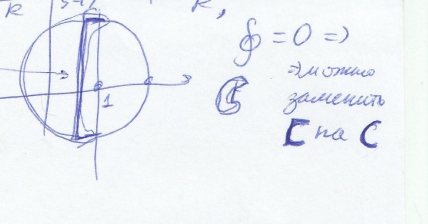
\includegraphics{p1.png}\q\\
\item $J(u) =  \frac{1}{2\pi i R} \IL_{[} f_u(s) u^{s-1} \os \frac{s-1}{R} + \frac{R}{s-1}  \cs ds $\\
$\lim\limits_{u\to\infty} J(u) = 0$\\
$g(s) = \frac{1}{2\pi i R}f(s)\os \frac{s-1}{R} + \frac{R}{s-1}    \cs $ ограничено на контуре, значит $\IL_{\TE+iR}^{1+iR}g(s) u^{s-1}ds \le \frac{\varepsilon}{\delta} $\\
Значит $|\IL_{BC} g(s)u^{s-1}ds |\le M2Ru^{\TE-1}\to0, u\to\infty\Ra \lim\limits_{u\to\infty}f_u(1) = f(1)\Ra $ интеграл сходится $\Ra$ асимптотический закон. $\pe$
\end{enumerate}
\end{mybox}



\newpage
\begin{mybox}{\hypertarget{bil8}{Билет 8}}
Доказательство асимптотического распределения распределения простых чисел. Асимптотическая формула $n$-го простого числа.\\\q\\
\begin{enumerate}
    \item
\begin{utv} $f(s) = -\frac{\zeta'(s)}{\zeta(s)} - \frac{1}{s-1} $ аналитическая при $\sigma \ge 1$
\end{utv}
$\pb$ Интересует $\sigma = 1$, т.к. при $\sigma > 1$ все ок.\\
$\exists$ окрестность, в которой функция аналитична.\\
$\zeta(s) = \frac{1}{s-1} + g(s),\q g(s)$  аналитичная.\\
$-\frac{-\zeta(s)}{s\zeta(s)} = -\frac{-\frac{1}{(s-1)^2} + g'(s)}{s\os \frac{1}{s-1} + g(s) \cs} = \frac{1}{s-1} \cdot \frac{1 - \overbrace{(s-1)^2}^{\to 0} g'(s)}{s (1 + (s-1)g(1))} = \frac{1}{s-1} + f(s)$, в $s = 1$ полюс первого порядка.$\pe$
\item Из преобразования Абеля $\sigma > 1$: $-\frac{\zeta'(s)}{\zeta(s)} - \frac{1}{s-1} = \IL_1^\infty\frac{\SI(x) - x}{x^{s+1}}dx\Ra f(s) = \IL_1^\infty\frac{\SI(x) - x}{x^{s+1}}dx $\\\q\\
\item $f_u(s) = \IL_1^u frac{\SI(x) - x}{x^{s+1}}dx$ -- целая, $u > 1$\\
$\pb  1) \IL_a^b \frac{dx}{x^{s+k}} = \left.\frac{x^{-s-k+1}}{-s-k+1} \right|_a^b = \frac{b^{-s-k+1} - a^{-s-k+1}}{-s-k+1} = \frac{1 + (-s-k+1)\ln(b) + (-s-k+1)^2g(s) -1 - (-s-k+1)\ln(a)}{-s-k+1} $ -- нет особенностей, значит целая. ($\pm 1 $ сокращаются, а дальше числитель делится на знаменатель ура).$\pe$
\item Считаем вычет $\frac{1}{2\pi i R}\cdot \oint\limits_{\Gamma(\TE,R)}(f(s) - f_u(s)) u^{s-1}\os \frac{s-1}{R} + \frac{R}{s-1}  \cs ds = \frac{1}{R}\cdot (f(1) - f_u(1)) \cdot 1 \cdot R $
\item $\left| \frac{1}{2\pi i R} \IL_{C_R}F_k(s)ds \right| \le \frac{B}{R};\q\SI(x) \le Cx, |\SI(x) - x|\le (C+1)x = Bx$\\
$\pb |f(s) - f_u(s)| = \left| \IL_u^\infty \frac{\SI(x) - x}{x^{s+1}}dx   \right| \le \IL_u^\infty \frac{Bx}{x^{s+1}}dx = \left.B\frac{x^{1-\sigma}}{1-\sigma}\right|_u^\infty = \frac{Bu^{1-\sigma}}{\sigma - 1}  $\\
$\Ra \left| \frac{s-1}{R} + \frac{R}{s-1}  \right| = 2 |Re\frac{s-1}{R}| = 2 \frac{\sigma - 1}{R} \pe$
\item $\left| \frac{1}{2\pi i R}\IL_[ f_u(s)u^{s-1} \os   \frac{s-1}{R} + \frac{R}{s-1} \cs   \right| \le \frac{B}{R}$\\
При этом можно заменить [ на (, т.к. интеграл по ([ равен 0.\\
$|f_u(s)| = |\IL_1^u \frac{\SI(x)-x}{x^{s+1}}dx|\le B \frac{u^{1-\sigma}}{1-\sigma}$\\
$|  \frac{s-1}{R} + \frac{R}{s-1} | = 2 |Re \frac{s-1}{R}| = 2 \frac{1 - \sigma}{R}$
\item Рассмотрим $J(u) = \frac{1}{2\pi i R} \IL_[ f(s)u^{s-1} \os   \frac{s-1}{R} + \frac{R}{s-1} \cs ds$\\
Утверждается что предел равен 0.\\
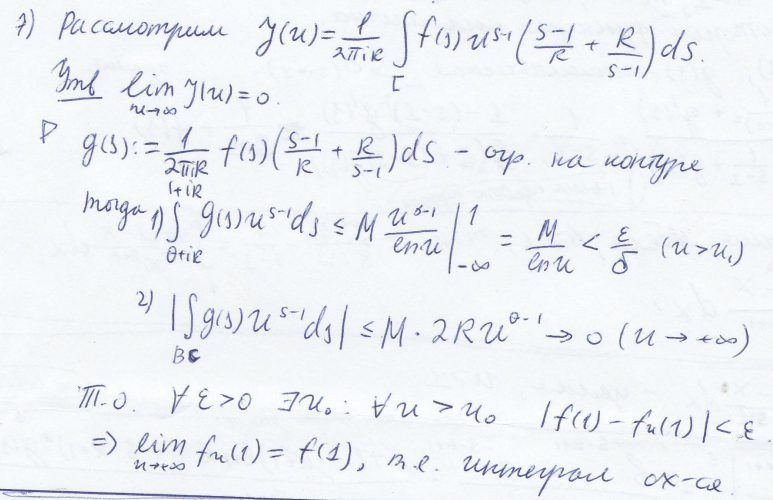
\includegraphics{p2.png}\q\\
\end{enumerate}
\begin{utv} $p_n \sim n\ln(n)$ -- закон распределения $n$-того простого.
\end{utv}
$\pb n = \pi(p_n) = \frac{p_n}{\ln(p_n)}(1+\alpha_n) $\\
$\ln(n)  = \ln(p_n) - \ln(\ln(p_n)) + \ln(1+\alpha_n) = \ln(p_n)(1 + \beta_n)  $\\
$\Ra n\ln(n) = p_n(1 + \alpha_n)(1 + \beta_n) \pe $
\end{mybox}



\newpage
\begin{mybox}{\hypertarget{bil9}{Билет 9}}
Простейшие свойства сравнений. Группа $\os Z/mZ \cs ^*$. Теорема Эйлера. Малая теорема Ферма. Элементарные доказательства бесконечности множества простых чисел в прогрессиях вида $4n+1$ и $4n+3$.\\\q\\
\begin{deff}[Сравнения]\q\\
$a \ee b \pmod{m}\iff m|(a-b) \iff a$ и $b$ дают одинаковые остатки при делении на $m$
\end{deff}
Свойства:
\begin{enumerate}
\item[0.] $a \ee b \pmod{m}\iff b \ee a \pmod{m}$
\item $a \ee b \pmod{m}\iff a + c \ee b + c\pmod{m}$
\item $a \ee b \pmod{m}\Ra ac \ee bc \pmod{m}$ !!!ТОЛЬКО В ОДНУ СТОРОНУ!!!
\item $\begin{cases} a \ee b \pmod{m}\\ c\ee d\pmod{m}\end{cases} \Ra a+c\ee b + d\pmod{m}$
\item $\begin{cases} a \ee b \pmod{m}\\ c\ee d\pmod{m}\end{cases} \Ra ac\ee bd\pmod{m}$
\item $ac\ee bc\pmod{mc}\Ra a\ee b\pmod{m}$
\item $ac\ee bc\pmod{m}, (m,c) = 1\Ra a\ee b\pmod{m}$
\end{enumerate}
Уравнение в факторкольце.\\
$\bb{Z}/m\bb{Z} = \{\bar{a}: \bar{a} = a + mt, t\in\bb{Z}\} \q\q a\ee b \iff \bar{a} = \bar{b}$\\
$\os \bb{Z}/m\bb{Z}  \cs^* = \{\bar{a}: \bar{a} = a + mt, (a,m) = 1\}$ !!ЭТО НЕ КОЛЬЦО, (т.к. нет сложения)!!! Но это группа по умножению: $1) \exists 1, 2) \exists a^{-1}$
\begin{lem} $ax\ee b\pmod{m}, (a,m) = 1\Ra \exists!c<m:x\ee c\pmod{m}$
\end{lem}
$\pb 1) ax\ee b\pmod{m} $\\
$\exists u,v: au+mv = 1\Ra au \ee 1 \pmod{m} $\\
$a(bu) \ee b\pmod{m}$\\
$x\ee c\ee bu\pmod{m}$\\
$2)$ пусть их два разных:$x_1\not= x_2$\\
$ax_1\ee b\pmod{m}, ax_2\ee b\pmod{m}\Ra ax_1 \ee ax_2\pmod{m}\Ra x_1\ee x_2\pmod{m}\pe$

\begin{teo}[Теорема Эйлера] $(a,m) = 1\Ra a^{\FI(m)} \ee 1\pmod{m}$
\end{teo}
\begin{teo}[Малая теорема Ферма] $p$-простое, $(p,a) = 1\Ra a^{p-1} \ee 1\pmod{p}$
\end{teo}
\begin{utv} $p|(a^2+b^2), p\not|a, p\not=2 \Ra p = 4m+1$
\end{utv}
$\pb a^2 + b^2 \ee 0\pmod{p}$\\
$a^2 \ee -b^2\pmod{p}, (a^2)^{\frac{p-1}{2}} \ee (b^2)^{\frac{p-1}{2}}\pmod{p}$\\
$a^{p-1}\ee b^{p-1} (-1)^{\frac{p-1}{2}} \Ra 1 \ee (-1)^{\frac{p-1}{2}}\pmod{p}\Ra \frac{p-1}{2} = 2m\Ra p = 4m+1\pe$
\begin{utv} Бесконечность множества простых вида $4n-1$.
\end{utv}
$\pb $ Пусть их конечное число. Пусть $p_n$ -- максимальное из них.\\
Рассмотрим $p = 4(p_1\cdots p_n) - 1$ не простое. $\exists q|p:q = 4k-1$, т.к. если все делители имеют вид $4k+1$, то и $p \ee 1 \pmod{4}$, но $q \not= p_j$ противоречие.$\pe$
\begin{utv} Бесконечность множества простых вида $4n+1$.
\end{utv}
$\pb $ Пусть $p_1,\dots,p_n$ -- все простые числа такого вида.\\
$(2p_1\cdots p_n)^2 + 1^2 = q_1\cdots q_m \Ra q_i = 4m_i+1$ по лемме, значит $q_i = p_j$ -- противоречие.$\pe$ 
\end{mybox}


\newpage
\begin{mybox}{\hypertarget{bil10}{Билет 10}}
Простейшие свойства групповых характеров. Построение характеров. Вычисление сумм $\sum_{a\in G} \chi(a)$ и $\sum_\chi \chi(a)$ для характеров $\chi$ группы $G$. Определение и свойства числовых характеров.\\\q\\
\begin{deff} [Определение характера]\q\\
Пусть $G$ -- конечная группа, коммутативная по умножению.\\
$\chi:G\to\bb{C}$ -- характер
\begin{enumerate}
\item $\chi(g) \not\ee0 $
\item $\chi(g_1 \cdot g_2) = \chi(g_1)\cdot \chi(g_2)  $
\end{enumerate}
\end{deff}
Свойства характеров.
\begin{enumerate}
\item $\chi(e) = 1\q\q \pb \chi(e\cdot e) = \chi(e)\cdot \chi(e) \pe$
\item $g^h=e\Ra (\chi(g))^h = 1 \Ra $ характеры принимают значения только корней из 1.
\item $\chi(g^{-1}) = \frac{1}{\chi(g)}$
\item $\chi_0(g)\ee 1$ -- главный характер.
\item $\chi_1 \chi_2 (g):= \chi_1(g)\cdot\chi_2(g)$
\end{enumerate}
Характеры образуют группу.
$\pb$
\begin{enumerate}
\item $\chi_1\chi_2 (g_1 g_2) = \chi_1(g_1)\chi_1(g_2)\chi_2(g_1)\chi_2(g_2) = \chi_1\chi_2(g_1)\chi_1\chi_2(g_2)$
\item $\exists \chi^{-1}: \chi^{-1}(g) =\chi(g^{-1}) = \frac{1}{\chi(g)}$
\item $\exists 1: \chi\chi^{-1}(g) = 1$
\end{enumerate}
Пусть $G = G_1\otimes \cdots \otimes G_n$, где все $G_i$ циклические. $ord g_i = h_i$\\
$ord G = h = h_1\cdots h_n$\\
$\forall g\in G g = g_1^{r_1}\cdots g_n^{r_n},\q\q 0\le r_i\le h_i$ и такое представление единственно.\\
Рассмотрим набор корней из 1:$\zeta_1,\dots,\zeta_n: \zeta_i^{h_i} = 1$\\
$\chi(g) = \zeta_1^{r_1}\cdots \zeta_n^{r_n}$
\begin{utv} Это характер и любой характер можно записать так.
\end{utv}
$\pb 1) g = g_1^{k_1}\cdots g_n^{k_n}\q\q k_j = r_j + a_jh_j\Ra g = g_1^{r_1}\cdots g_n^{r_n} $ а дальше рассмотрим характер и такие ого записался.\\
$2) a = g_1^{a_1}\cdots g_n^{a_n};\q b = g_1^{b_1}\cdots g_n^{b_n}$\\
$ab = g_1^{a_1 + b_1}\cdots g_n^{a_n + b_n}$ и получаем что характер произведения равен произведению характеров. Проверили. $\pe$\\\q\\
Если $\chi \not=\chi_0$, то $\exists g: \chi(g) \not=1$\\
Если $g\not=e$, то $\exists \chi: \chi(g)\not=1$
\begin{utv}\q\\
\begin{enumerate}
\item $S = \SL_{g\in G}\chi(g) = \begin{cases}h, \chi = \chi_0\\ 0, \chi \not= \chi_0\end{cases}$
\item $\sigma = \SL_{\chi}\chi(g) = \begin{cases}h, g = e\\ 0, e \not= e\end{cases}$
\end{enumerate}
\end{utv}
$\pb$ Сначала рассмотрим тривиальные случаи:\\
$\chi = \chi_0\Ra\chi(g) = 1\Ra S = |G| = h$\\
$g = e\Ra \chi(e) = 1\Ra\sigma = |G| = h$\\
Теперь остальные:\\
$\chi \not=\chi_0 \Ra \exists a\in G: \chi(a)\not=1$\\
$\chi(a)S = \SL_{g\in G}\chi(a)\chi(g) = S\Ra (\chi(a) - 1) S = 0 \Ra S = 0$\\\q\\
$g\not=e\Ra\exists \chi_1:\chi_1(g)\not=1$\\
$\chi_1(g)\sigma = \sigma \Ra \sigma = 0 \pe$

Числовые характеры.\\
$\bb{Z}_m^* = \os \bb{Z}/m\bb{Z}  \cs^* = \{\bar{a}: \bar{a} = a + mt,\q (a,m) = 1 \}, \bar{a}\bar{b} = \overline{ab}  $\\
$\chi(x) = \begin{cases} \chi(\bar{x}), (x,m)=1\\0,(x,m) \not=1 \end{cases} $\\
$\chi_0(x) = \begin{cases} 1, (x,m)=1\\0,(x,m) \not=1 \end{cases} $\\\q\\
$a\ee b \pmod{m} \Ra \chi(a) = \chi(b) $\\
$\chi(ab) = \chi(a)\chi(b) $\\
$\chi(a)\not=0 \iff (a,m)=1$\\\q\\
$\SL_{x=1}^m \chi(x) = \begin{cases} \FI(m), \chi = \chi_0\\0 \end{cases} $\\
$\SL_{\chi} \chi(x) = \begin{cases} \FI(m), x = 1\\0 \end{cases} $\\
$|\SL_{x=1}^{mq+r} \chi(x) | = |\SL_{x=mq+1}^{mq+r} \chi(x)|\le r\le m$
\end{mybox}





\newpage
\begin{mybox}{\hypertarget{bil11}{Билет 11}}
Аналитичность функции Дирихле $L(s,\chi)$ в области $\sigma > 1$. Разложение в ряд Дирихле ее логарифмической производной. Отсутствие нулей $L$-функции в области $\sigma > 1$. Представление $L$-функции в виде бесконечного произведения. Аналитическое продолжение функции $L(s,\chi_0)$ в область $\sigma > 0$.\\\q\\
\begin{deff}
$L(s,\chi) = \SL_{n=1}^\infty \frac{\chi(n)}{n^s}$ -- функция Дирихле.
\end{deff}
$\zeta(s) = \SL_{n=1}^\infty \frac{1}{n^s};$ если $\SL_{n=1}^\infty f(n) = A, \SL_{d=1}^\infty f(d)\Lambda(d) = B$ -- абсолютно сходящийся ряд. $\Lambda(n) = \begin{cases} \ln(p), n=p^k\\0  \end{cases} \q\q \Ra AB = \SL_{n=1}^\infty f(n)\ln(n)$\\\q\\
$\SL_{n=1}^\infty f(n) = \prod\limits_p \os 1 - f(p)\cs^{-1}$ Если $f(n) = \frac{\chi(n)}{n^s}\Ra L(s,\chi) = \prod\limits_p \os 1 - \frac{\chi(p)}{p^s}   \cs^{-1} $\\
$L(s,\chi) \cdot \SL_{n=1}^\infty \frac{\chi(n)\Lambda(n)}{n^s} = \SL_{n=1}^\infty \frac{\chi(n)\ln(n)}{n^s}  = -L'(s,\chi)\Ra $ в области $\sigma > 1: L(s,\chi)\not=0$\\
$\chi_0(p) = \begin{cases} 1, (m,p) = 1\\0  \end{cases}\Ra L(s,\chi) = \prod\limits_{p\not|m}(1 - \frac{1}{p^s})^{-1} $\\
$L(s,\chi_0) = \zeta(s) \prod\limits_{p|m} (1 - \frac{1}{p^s})^{-1} = \os \frac{1}{s-1} + f(s) \cs  \prod\limits_{p|m} (1 - \frac{1}{p^s})^{-1} = \frac{a_m}{s-1} + f_m(s),\q\q a_m = \prod\limits_{p|m} (1 - \frac{1}{p^s}) = \frac{\FI(m)}{m} > 0 \Ra  L(s,\chi_0)$  аналитична в области $\sigma > 0$
\end{mybox}


\newpage
\begin{mybox}{\hypertarget{bil12}{Билет 12}}
Теорема о почленном дифференцировании ряда Дирихле. Область аналитичности функции $L(s, \chi)$ при $\chi \not= \chi_0$.\\\q\\
Рассмотрим область $D(\delta, \TE) = \begin{cases} \sigma > \delta > 0\\|arg(s)| < \TE, \TE \in (0, \frac{\pi}{2})\end{cases}$\\
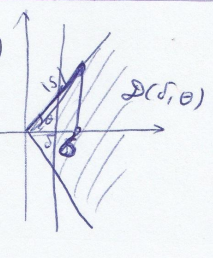
\includegraphics{p3.png}\q\\
\begin{utv}\q\\
\begin{enumerate}
\item Ряд $\SL_n \frac{a_n}{n^s} $ равномерно сходится в $D(\delta, \TE)$
\item $f(s)$ аналитична в области $\sigma > 0,$ где $f(s) = \SL_n\frac{a_n}{n^s}$
\end{enumerate}
\end{utv}
$\pb$ Определение равномерной сходимости: $\forall \varepsilon > 0 \exists M(\varepsilon): \forall N > M, \forall s\in D(\delta, \TE): |R_N(s)| = |\SL_{n = N+1}^\infty \frac{a_n}{n^s}| < \varepsilon$\\
Перепишем: $R_N(s) = \SL_{k=0}^\infty \frac{a_{N+k}}{(N+k)^s}\q\q A(x) = \SL_{k\le x}a_k; g(x) = \frac{1}{(N+x)^s}$\\
$|A(x)| \le 2C; \q g(x) \to 0\Ra A(x)g(x)\to0$\\
$g'(x) = -s(N+x)^{-s-1}, s\IL_1^\infty A(t)(N+t)^{-s-1}dt $ сходится, значит можно использовать преобразование Абеля.\\
$\SL_{k=1}^\infty g(k) a_k = -\IL_1^\infty A(t) g'(t) dt = -s\IL_1^\infty A(t)(N+t)^{-s-1}dt = R_N(s) $\\
$|R_N(s)| \le |s|\IL_1^\infty 2C(N+t)^{-s-1}dt = |s| \cdot 2C\left.\frac{(N+t)^{-\sigma}}{-\sigma}\right|_1^\infty = 2C\frac{(N+1)^{-\sigma}}{\sigma}|s|$\\
В области $D(\delta, \TE): \q\q |R_N(s)|\le 2CN^{-\delta}\frac{1}{\cos(\TE)} < \varepsilon \Ra$ выполняется равномерная сходимость.\\
Для любой точки правее нуля можно подобрать такие $\delta$ и $\TE$, чтобы она попала в область. Раз в таких областях ряд сходится равномерно, значит его можно дифференцировать бесконечное число раз, значит функция аналитична.$\pe$

\end{mybox}





\newpage
\begin{mybox}{\hypertarget{bil13}{Билет 13}}
Теорема об области сходимости ряда Дирихле с неотрицательными коэффициентами.\\\q\\
Пусть есть  ряд $f(s) = \sum a_n n^{-1}, \q \sigma_1 < \sigma_2 < \sigma_0$\\
\begin{teo} Пусть функция $f(s):$
\begin{enumerate}
\item $f(s)$ аналитична при $\sigma > \sigma_1$
\item $f(s) = \SL_{n=1}^\infty  \frac{a_n}{n^s},\q(\sigma > \sigma_2) $
\item $a_n \ge 0$
\end{enumerate}
Тогда $f(s)$ раскладывается в ряд Дирихле при $\sigma > \sigma_1$ и его можно почленно дифференцировать. $///<WTF?$
\end{teo}
$\pb $ Если $f(s) \sum \frac{a_n}{n^s}$ сходится при $s = s_0 = \sigma_0 + it_0$, то ряд Дирихле задаёт функцию, аналитичную в области $\sigma > \sigma_0\Ra$ можно дифференцировать.\\
$\Ra$ есть прямая, разделяющая области сходимости и расходимости.\\
Рассмотрим $\sigma_0 > \sigma_2$,  разложим в ряд Тейлора:\\
$f(s) = \SL_{k=0}^\infty \frac{f^{(k)}(\sigma_0)}{k!} (s - \sigma_0)^k $\\
Берем $\sigma\in(\sigma_1, \sigma_2)$ и подставляем вместо $s$. (анализируем сходимость в $\sigma > \sigma_1$)\\
$f(\sigma) = \SL_{k=0}^\infty \frac{f^{(k)}}{k!}(\sigma - \sigma_0)^k = \SL_{k=0}^\infty \SL_{n=1}^\infty \frac{a_n (-\ln(n))^k}{n^{\sigma_0}} \frac{1}{k!} (\sigma - \sigma_0)^k   = \SL_{k=0}^\infty \frac{(\sigma - \sigma_0)^k}{k!}\SL_{n=1}^\infty \frac{a_n (-\ln(n))^k}{n^{\sigma_0}} = \SL_{n=1}^\infty \frac{a_n}{n^{\sigma_0}} \SL_{k=0}^\infty \frac{\os(\sigma_0 - \sigma)\ln(n)\cs^k}{k!}  = \SL_{n=1}^\infty \frac{a_n}{n^{\sigma_0}} e^{(\sigma - \sigma_0)\ln(n)} = \SL_{n=1}^\infty \frac{a_n}{n^\sigma} $\\
Ряд задает аналитическую функцию по теореме единственности аналитического продолжения функции заданной этим рядом при $\sigma > \sigma_1 \pe$
\end{mybox}



\newpage
\begin{mybox}{\hypertarget{bil14}{Билет 14}}
Неравенство $L(1,\chi)\not=0$ для действительного характера $\chi$.\\\q\\
\begin{deff} Характер $\chi$ действительный, если $\chi^2 = \chi_0 = 1$
\end{deff}
\begin{lem} $f(s):= \zeta(s) L(s,\chi) \Ra$
\begin{enumerate}
\item $f(s) = \SL_{n=1}^\infty \frac{a_n}{n^s},\q\sigma > 1 $
\item $a_n \ge 0$
\item $a_{n^2} \ge 1$
\item $\SL_{n=1}^\infty \frac{a_n}{\sqrt{n}} $ расходится.
\end{enumerate}
\end{lem}
$\pb f(s) = \SL_{k=1}^\infty \frac{1}{k^s}  \SL_{d=1}^\infty \frac{\chi(d)}{d} = \SL_{n=1}^\infty \frac{1}{n^s} \SL_{d|n}\chi(d)$\\
Если $n = p_1^{k_1}\cdots p_r^{k_k}$, то $a_n = \SL_{d|n}\chi_d  \prod\limits_{j=1}^n (1 + \chi(p_j) + \chi(p_j^2) + \cdots)  = \prod\limits_{j=1}^n (1 + \chi(p_j) + \chi(p_j^2) + \cdots) =  \prod\limits_{j=1}^n (1 + \chi(p_j) + \chi^2(p_j) + \cdots)$\\
где $a_{n_j} = \begin{cases} 1, \chi(p_j) = 0\\k_j + 1, \chi(p_j)=1\\1, \chi(p_j) = -1, k_j\%2==0\\0  \end{cases}$\\
Если $n = k^2,$ то все $k_j \%2==0\Ra$\\
$\prod\limits_{j=1}^r  a_{n_j} \ge 1 \Ra 1)+2)+3)$ ////<WTF??\\
$4) \SL_{n=1}^\infty \frac{a_n}{\sqrt{n}} \ge \SL_{k=1}^\infty \frac{a_{k^2}}{k}  \Ra$ расходится. $\pe$

\begin{teo} $\chi$-- действительный характер, тогда $L(1, \chi) \not=0$
\end{teo}
$\pb L(1,\chi) = 0\Ra L(s\chi) = (s-1)g(s), \q g(s)$ аналитичная\\
$\zeta(s) =\frac{1}{s-1} + h(s) $ -- тоже аналитичная\\
$f(s) = \zeta(s) L(s,\chi) = g(s) + g(s)h(s)(s-1)  $ представляется сходящимся рядом Дирихле в $\sigma > 0$ а это противоречие с пунктом 4 леммы $\pe$ 
\end{mybox}





\newpage
\begin{mybox}{\hypertarget{bil15}{Билет 15}}
Неравенство $L(1,\chi)\not=0$ при $\chi^2\not=\chi_0$.\\\q\\
\begin{lem} Пусть $s\in \bb{R}, s > 1$, тогда $A:= |L^3(s,\chi_0)\cdot L^4(s,\chi)\cdot L(s, \chi^2)| \ge 1$
\end{lem}
$\pb L(s, \chi) = \prod\limits_p \os 1 - \frac{\chi(p)}{p^s} \cs ^{-1} $\\
$A = \prod\limits_{p|m} \left|\os 1 - \frac{1}{p^s} \cs^3  \os 1 - \frac{\chi(p)}{p^s} \cs^4  \os 1 - \frac{\chi^2(p)}{p^s} \cs^3  \right|^{-1}   $\\
Из \hyperlink{bil6}{билета 6} $|(1-r)^3 (1-re^{i\varphi})^4 (1 - re^{2i\FI})| \le 1 \q\q\Ra r = \frac{1}{p}\Ra \pe$

\begin{teo} При $\chi \not= \chi_0: L(1,\chi)\not=0$
\end{teo}
$\pb L(1,\chi) = 0\Ra L'(1,\chi) = \lim\limits_{s\to1+0} \frac{L(s,\chi) - L(1,\chi)}{s-1} = \lim\limits_{s\to1+}\frac{L(s,\chi)}{s-1}\Ra \left| \frac{L(s,\chi)}{s-1} \right| \le C_1$\\
$L(s, \chi_0) = \SL_{(m,n) = 1}^\infty \frac{1}{n^s} < \zeta(s) \le \frac{2}{s-1} $\\
$L(s,\chi) = (s-1)g_m(s) $\\
$|L(s,\chi)| \le C_1(s-1)\q\q |L(s,\chi^2)| \le C_2$\\
$1 \le A\le \left| \os  \frac{2}{s-1} \cs^3 (C_1 (s-1))^4 C_2  \right| \to 0$ противоречие. $\pe$

\end{mybox}



\newpage
\begin{mybox}{\hypertarget{bil16}{Билет 16}}
Доказательство теоремы Дирихле о бесконечности множества простых чисел в арифметической прогрессии.\\\q\\
\begin{teo}[Теорема Дирихле] Пусть $m\ge 2$. В прогрессии $mx+l, (m,l) = 1$ бесконечно много простых.
\end{teo}
$\pb F(s) = \SL_{\chi}\chi(u) \os -\frac{L'(s,\chi)}{L(s,\chi)}  \cs, \q\q s\in\bb{R}, s > 1 $\\
$u$ выбрали так, что $lu\ee 1\pmod{m}$\\
\begin{enumerate}
\item На $(1,2)\q F(s)$ не ограничена\\
$F(s) = -1 \frac{L'(s,\chi_0)}{L(s,\chi)} + \SL_{\chi\not=\chi_0} \chi(u) \frac{L'(s,\chi_0)}{L(s,\chi)}  = \frac{1}{s-1} + G(s),\q\q G(s) $ ограничена при $\sigma > 1$
\item Если количество простых конечно, то $F(s)$ ограничена на $(1,2)$\\
$-\frac{L'(s,\chi)}{L(s,\chi)} = \SL_{n=1}^\infty \frac{\Lambda(n)\chi(n)}{n^s}\Ra F(s) = \SL_{\chi} \chi(u) \SL_{n=1}^\infty \frac{\Lambda(n)\chi(n)}{n^s} = \SL_{n=1}^\infty \frac{\Lambda(n)}{n^s} \SL_\chi \chi(un) = \FI(m) \SL_{un\ee1\pmod{m}} \frac{\Lambda(n)}{n^s}  =  \FI(m) \SL_{n\ee l\pmod{m}} \frac{\Lambda(n)}{n^s} = \FI(m)\SL_{p\ee l\pmod{m}} \frac{\ln(p)}{p^s} + R(s)$\\
$0 \le R(s)  = \FI(m)\SL_{p}\SL_{k=2, p^k \ee l\pmod{m}}  \frac{\ln(p)}{p^s}\le \FI(m)  \SL_{p=2}^\infty \frac{\ln(p)}{p(p-1)} \le C $\\
То есть $F(s) = \FI(m) \SL_{p\ee l\pmod{m}} \frac{\ln(p)}{p(p-1)} + O(1) $\\
Если число простых конечно, то $F(s) $ ограничена. Противоречие.$\pe$
\end{enumerate}

\end{mybox}



\newpage
\begin{mybox}{\hypertarget{bil17}{Билет 17}}
Свойства минимального многочлена алгебраического числа. Целые алгебраические числа. Лемма Гаусса и ее следствия, относящиеся к целым алгебраическим числам.\\\q\\

\begin{deff} Число $\alpha\in\bb{C}$ -- алгебраическое, если $\exists A(x) = x^n + a_{n-1}x^{n-1} + \cdots + a_0, \q a_i\in\bb{Q}, \q\q A(\alpha) = 0$\\
Иначе число трансцендентное.
\end{deff}


\begin{deff} Минимальный многочлен числа $\alpha$ -- ненулевой многочлен минимальной степени, имеющий корень $\alpha$. // Далее считаем, что старший коэффициент $= 1$
\end{deff}
Свойства:
\begin{enumerate}
\item Единственность. $\pb deg(A_1(x) - A_2(x)) \le n-1 \Ra$ полученное -- не минимальный $\pe$
\item $B(x)\in\bb{Q}[x], \q B(\alpha) = 0\Ra A(x)|B(x)$\\
$\pb B(x) = A(x)Q(x) + R(x), deg(R) < deg(A)$\\
$B(\alpha) = \overbrace{A(\alpha)}^{=0}Q(\alpha) + R(\alpha)\Ra R(x) = 0\pe$
\item $A(x)\in\bb{Q}[x], A(\AL) = 0 \Ra$\q\q$A(x)$ минимальный многочлен для $\AL \iff A(x)$ неприводим над $\bb{Q}[x]$\\
$\pb \rightarrow$\\
$A(x) = A_1(x)A_2(x)\q\q 0 < deg(A_i) < deg(A)\Ra A_1(\AL) = 0$ или $A_2(\AL) = 0$, тогда $A(x)$ не минимальный.\\
$\leftarrow$\\
$A_0$ -- минимальный, $A(x)$ неприводимый $ = A_0 \cdot \underbrace{A_1}_{=const} = A_0(x)\pe$
\end{enumerate}

\end{mybox}


























\newpage

\section{Определения и формулировки}
\begin{deff2} $b|a$, если $\exists q\in \mathbb{Z}: a=bq$
\end{deff2}
\begin{teo2}[Основная теорема арифметики]\q\\
\begin{enumerate}
    \item всякое $a \in \bb{N}, a > 1$ представляется в виде $a = p_1\cdots p_n$, где $p_i$ простые.
    \item это представление единственно с точностью до порядка сомножителей.
\end{enumerate}
\end{teo2}

\begin{deff2} $a\in \bb{Z}, b\in\bb{N}\Rightarrow \exists ! q,r: \begin{cases} a = bq+r\\0 \le r < b\end{cases} $ --деление с остатком
\end{deff2}

\begin{teo2}[Теорема о представлении НОД]\q\\
$(a,b) = d \Ra \exists u,v\in\bb{Z}: d = au+bv$
\end{teo2}
\begin{utv2} Пусть $a = p_1^{k_1}\cdots p_n^{k_n}, b = p_1^{l_1}\cdots p_n^{l_n}$. Тогда $b|a\iff \forall i: l_i \le k_i$
\end{utv2}

\begin{utv2} $(a,b) = p_1^{s_1}\cdots p_n^{s_n}$, где $s_j = \min\{k_j, l_j\}$\\
$[a,b] = p_1^{t_1}\cdots p_n^{t_n},$ где $t_j = \max\{k_j, l_j\}$
\end{utv2}
\begin{teo2}[Теорема о бесконечности простых чисел]\q\\
Простых чисел бесконечно много.
\end{teo2}

\begin{lem2}
$0\le l_1 = l_2 = l_3 \le L_1 = L_2 = L_3 \le +\infty$
\end{lem2}

\begin{utv2} $f(x)$ неубывающая на $[1;\infty]\Ra$ если $\IL_1^\infty \frac{f(x) - x}{x^2}dx$ сходится то \\$f(x)\sim x, x\to\infty$
\end{utv2}
\begin{teo2}[Теорема Чебышева]\q\\
$\exists a.b > 0: \forall x \ge 2:\q a\frac{x}{\ln(x)} <\pi(x) <b\frac{x}{\ln(x)} $
\end{teo2}
\begin{teo2}[Теорема Эйлера]\q\\$\sum_p \frac{1}{p}$ расходится.
\end{teo2}
\begin{utv2} $\alpha n \ln(n) < p_n < \beta n \ln(n)   $
\end{utv2}

\begin{deff2}
Дзета-функция Римана: $s = \sigma + it, \zeta (s) := \SL_{n=1}^\infty \frac{1}{n^s}$
\end{deff2}

\begin{teo2}\q\\
$\sigma > 1: -\frac{\zeta'(s)}{\zeta(s)}  \SL_{n=1}^\infty \frac{\Lambda(n)}{n^s} $
\end{teo2}
\begin{lem2}\q\\
$f(n)$ -- вполне мультипликативная, $A = \SL_{k=1}^\infty f(k);\q\q B = \SL_{d=1}^\infty f(d)\Lambda(d)$ -- абсолютно сходятся. Тогда $AB = \SL_{n=1}^\infty f(n) ln(n)$
\end{lem2}
\begin{teo2}\q\\
В области $\sigma > 1: \zeta(s) = \prod\limits_p (1 - \frac{1}{p^s})^{-1}$
\end{teo2}
\begin{lem2}\q\\
$f(n)$ -- вполне мультипликативная, ряд $\sum f(n)$ абсолютно сходится $\Ra S = \SL_{n=2}^\infty f(n) = \prod\limits_p (1-f(p))^{-1}  $
\end{lem2}
\begin{teo2}
Преобразование Абеля. $\SL_{n\le x} a_n g(n), a_n\in \bb{C}, g(x)$ -- комплекснозначная функция действительного аргумента.\\
$x\in[1,+\infty); \exists$ непрерывная $g'(x), \SL_{n \le x}a_n = A(x)$\\
\begin{enumerate}
    \item $\SL_{n\le x}a_ng(n) = A(x)g(x) - \IL_1^x A(t)g'(t)dt $
    \item если $\lim\limits_{x\to\infty} A(x)g(x) = 0$, то $\SL_{n=1}^\infty a_ng(n) = \IL_1^\infty A(t)g'(t)dt $
\end{enumerate}
\end{teo2}


\begin{lem2} $\forall 0 < r < 1, \varphi\in \bb{R} \Ra M = \left| (1-r)^3(1-re^{i\varphi})^4 (1 - re^{2i\varphi}) \right| \le 1 $
\end{lem2}
\begin{lem2} При $\sigma > 1: |\zeta^3(\sigma)\zeta^4(\sigma+it)\zeta(\sigma+2it)| \ge 1$
\end{lem2}
\begin{teo2} При $\sigma \ge 1 \q \zeta(s) \not= 0$
\end{teo2}
\begin{teo2}[Асимптотический закон распределения простых чисел.]\q\\
$\pi(x)\sim \frac{x}{\ln(x)}, x\to\infty$
\end{teo2}
\begin{utv2} $f(s) = -\frac{\zeta'(s)}{zeta(s)} - \frac{1}{s-1} $ аналитическая при $\sigma \ge 1$
\end{utv2}
\begin{utv2} $p_n \sim n\ln(n)$ -- закон распределения $n$-того простого.
\end{utv2}
\begin{deff2}[Сравнения]\q\\
$a \ee b \pmod{m}\iff m|(a-b) \iff a$ и $b$ дают одинаковые остатки при делении на $m$
\end{deff2}
\begin{lem2} $ax\ee b\pmod{m}, (a,m) = 1\Ra \exists!c<m:x\ee c\pmod{m}$
\end{lem2}
\begin{teo2}[Теорема Эйлера] $(a,m) = 1\Ra a^{\FI(m)} \ee 1\pmod{m}$
\end{teo2}
\begin{teo2}[Малая теорема Ферма] $p$-простое, $(p,a) = 1\Ra a^{p-1} \ee 1\pmod{p}$
\end{teo2}
\begin{utv2} $p|(a^2+b^2), p\not|a, p\not=2 \Ra p = 4m+1$
\end{utv2}
\begin{utv2} Бесконечность множества простых вида $4n-1$.
\end{utv2}
\begin{utv2} Бесконечность множества простых вида $4n+1$.
\end{utv2}
\begin{deff2} [Определение характера]\q\\
Пусть $G$ -- конечная группа, коммутативная по умножению.\\
$\chi:G\to\bb{C}$ -- характер
\begin{enumerate}
\item $\chi(g) \not\ee0 $
\item $\chi(g_1 \cdot g_2) = \chi(g_1)\cdot \chi(g_2)  $
\end{enumerate}
\end{deff2}

\begin{utv2}
\begin{enumerate}
\item $S = \SL_{g\in G}\chi(g) = \begin{cases}h, \chi = \chi_0\\ 0, \chi \not= \chi_0\end{cases}$
\item $\sigma = \SL_{\chi}\chi(g) = \begin{cases}h, g = e\\ 0, e \not= e\end{cases}$
\end{enumerate}
\end{utv2}

\begin{deff2}
$L(s,\chi) = \SL_{n=1}^\infty \frac{\chi(n)}{n^s}$ -- функция Дирихле.
\end{deff2}

\begin{utv2}\q\\
\begin{enumerate}
\item Ряд $\SL_n \frac{a_n}{n^s} $ равномерно сходится в $D(\delta, \TE)$
\item $f(s)$ аналитична в области $\sigma > 0,$ где $f(s) = \SL_n\frac{a_n}{n^s}$
\end{enumerate}
\end{utv2}
\begin{teo2} Пусть функция $f(s):$
\begin{enumerate}
\item $f(s)$ аналитична при $\sigma > \sigma_1$
\item $f(s) = \SL_{n=1}^\infty  \frac{a_n}{n^s},\q(\sigma > \sigma_2) $
\item $a_n \ge 0$
\end{enumerate}
Тогда $f(s)$ раскладывается в ряд Дирихле при $\sigma > \sigma_1$ и его можно почленно дифференцировать.
\end{teo2}
\begin{deff2} Характер $\chi$ действительный, если $\chi^2 = \chi_0 = 1$
\end{deff2}
\begin{lem2} $f(s):= \zeta(s) L(s,\chi) \Ra$
\begin{enumerate}
\item $f(s) = \SL_{n=1}^\infty \frac{a_n}{n^s},\q\sigma > 1 $
\item $a_n \ge 0$
\item $a_{n^2} \ge 1$
\item $\SL_{n=1}^\infty \frac{a_n}{\sqrt{n}} $ расходится.
\end{enumerate}
\end{lem2}
\begin{teo2} $\chi$-- действительный характер, тогда $L(1, \chi) \not=0$
\end{teo2}
\begin{lem2} Пусть $s\in \bb{R}, s > 1$, тогда $A:= |L^3(s,\chi_0)\cdot L^4(s,\chi)\cdot L(s, \chi^2)| \ge 1$
\end{lem2}

\begin{teo2} При $\chi \not= \chi_0: L(1,\chi)\not=0$
\end{teo2}


\begin{teo2}[Теорема Дирихле] Пусть $m\ge 2$. В прогрессии $mx+l, (m,l) = 1$ бесконечно много простых.
\end{teo2}



\begin{deff2} Число $\alpha\in\bb{C}$ -- алгебраическое, если $\exists A(x) = x^n + a_{n-1}x^{n-1} + \cdots + a_0, \q a_i\in\bb{Q}, \q\q A(\alpha) = 0$\\
Иначе число трансцендентное.
\end{deff2}


\begin{deff2} Минимальный многочлен числа $\alpha$ -- ненулевой многочлен минимальной степени, имеющий корень $\alpha$. // Далее считаем, что старший коэффициент $= 1$
\end{deff2}

\end{document}




